\documentclass[conference]{IEEEtran}
\IEEEoverridecommandlockouts
% The preceding line is only needed to identify funding in the first footnote. If that is unneeded, please comment it out.
\usepackage{cite}
\usepackage{amsmath,amssymb,amsfonts}
\usepackage{algorithmic}
\usepackage{graphicx}
\usepackage{textcomp}
\usepackage{xcolor}
\def\BibTeX{{\rm B\kern-.05em{\sc i\kern-.025em b}\kern-.08em
    T\kern-.1667em\lower.7ex\hbox{E}\kern-.125emX}}
\begin{document}

\title{Conference Paper Title}

%% TODO add authors here %%
%\author{\IEEEauthorblockN{1\textsuperscript{st}Gabriele Monaco}
%\IEEEauthorblockA{\textit{Department of Electronic and Information Technology} \\
%\textit{Technical University of Kaiserslautern}\\
%Kaiserslautern, Germany \\
%monaco@rhrk.uni-kl.de}
%\and
%\IEEEauthorblockN{2\textsuperscript{nd} Given Name Surname}
%\IEEEauthorblockA{\textit{dept. name of organization (of Aff.)} \\
%\textit{name of organization (of Aff.)}\\
%City, Country \\
%email address or ORCID}
%\and
%\IEEEauthorblockN{3\textsuperscript{rd} Given Name Surname}
%\IEEEauthorblockA{\textit{dept. name of organization (of Aff.)} \\
%\textit{name of organization (of Aff.)}\\
%City, Country \\
%email address or ORCID}
%}

\maketitle

\begin{abstract}
    Various application are relying on location for various purposes in their activity, in general users need to be advertise their own position to the server and can then spoof it. This can be dangerous in many contexts, from secure networks to aircraft. In this paper we are going to discuss about how to securely verify the location in wireless networks by exploiting physical properties of the incoming signals. It is indeed possible to determine, based on some measured parameters, if a location claim can be trustworthy and there are several methods how to do that. We are going through some of the physical property that can be exploited for this purpose, pointing out advantages and disadvantages of the various approaches.
\end{abstract}

\begin{IEEEkeywords}
component, formatting, style, styling, insert
\end{IEEEkeywords}

\section{Mobility}

%% write here %%

%\subsection{Introduction}

In the following section we will discuss about the situation when the prover is moving, here some physical properties of the resulting signal may be exploited to verify it's actual location (or track, since many locations can be verified during time). We will talk about prover to reference either a moving object whose position (and movement) needs to be verified and an attacker who is not moving (speed vector = \(\vec{0}\)) and is trying to spoof its location. The prover is periodically sending location claims (sometimes referred as beacons) which are simple signals sent at a defined frequency. They contain information about the absolute position and absolute speed of the object, a timestamp of when the message has been sent is also included. Naturally, we are considering a potential attacker to be able to send any value in its messages, hence all the values contained in a claim need to be verified and cannot be trusted a priori. The verifiers are simple stationary receivers which are aware of their own position and which can exchange messages with one another (to verify claims in a distributed way, for instance), the attacker may know the verifiers positions and in general there's no limit in its knowledge.

\subsection{Mobility Differentiated Time of Arrival}

When it comes to a moving prover, the principle of Time of Arrival (ToA) can be extended to Mobility-differentiated ToA (MDToA), according to this paradigm described in details in \cite{schaefer15}, over the time many beacons are collected from the prover, all of them containing informations about claimed position and speed. The verifier(s) can then compute according to a mathematical model the expected time of arrival of those messages (according to claimed parameters). If such a computation differs from the measured value, the verifier is able to detect a scam. Rather than \textit{location verification}, we can refer here as \textit{track verification}, since the prover is actually moving and we are going to verify its position over time, hence drawing a track.

In details, we define the propagation delay \(D_i\) as stated in formula \eqref{gm_delay}. Now we can say that the claim is trustworthy if the measured delay (\(D_{i,j}^m\)) between two beacons (here \textit{i} and \textit{j}) is equal to the claimed delay (obtained as difference of the claimed timestamps) plus the individual measured delays (see equation \eqref{gm_delay_trust} and figure \ref{gm_delay_pic}) \cite{schaefer15}.

\begin{equation}
    D_i = \frac{d_i}{c}
    \label{gm_delay}
\end{equation}
\emph{The time delay is obtained by dividing the absolute distance by the speed of light}

\begin{equation}
    D_{i,j}^m = D_{i,j} + (D_j - D_i)
    \label{gm_delay_trust}
\end{equation}

\begin{figure}
    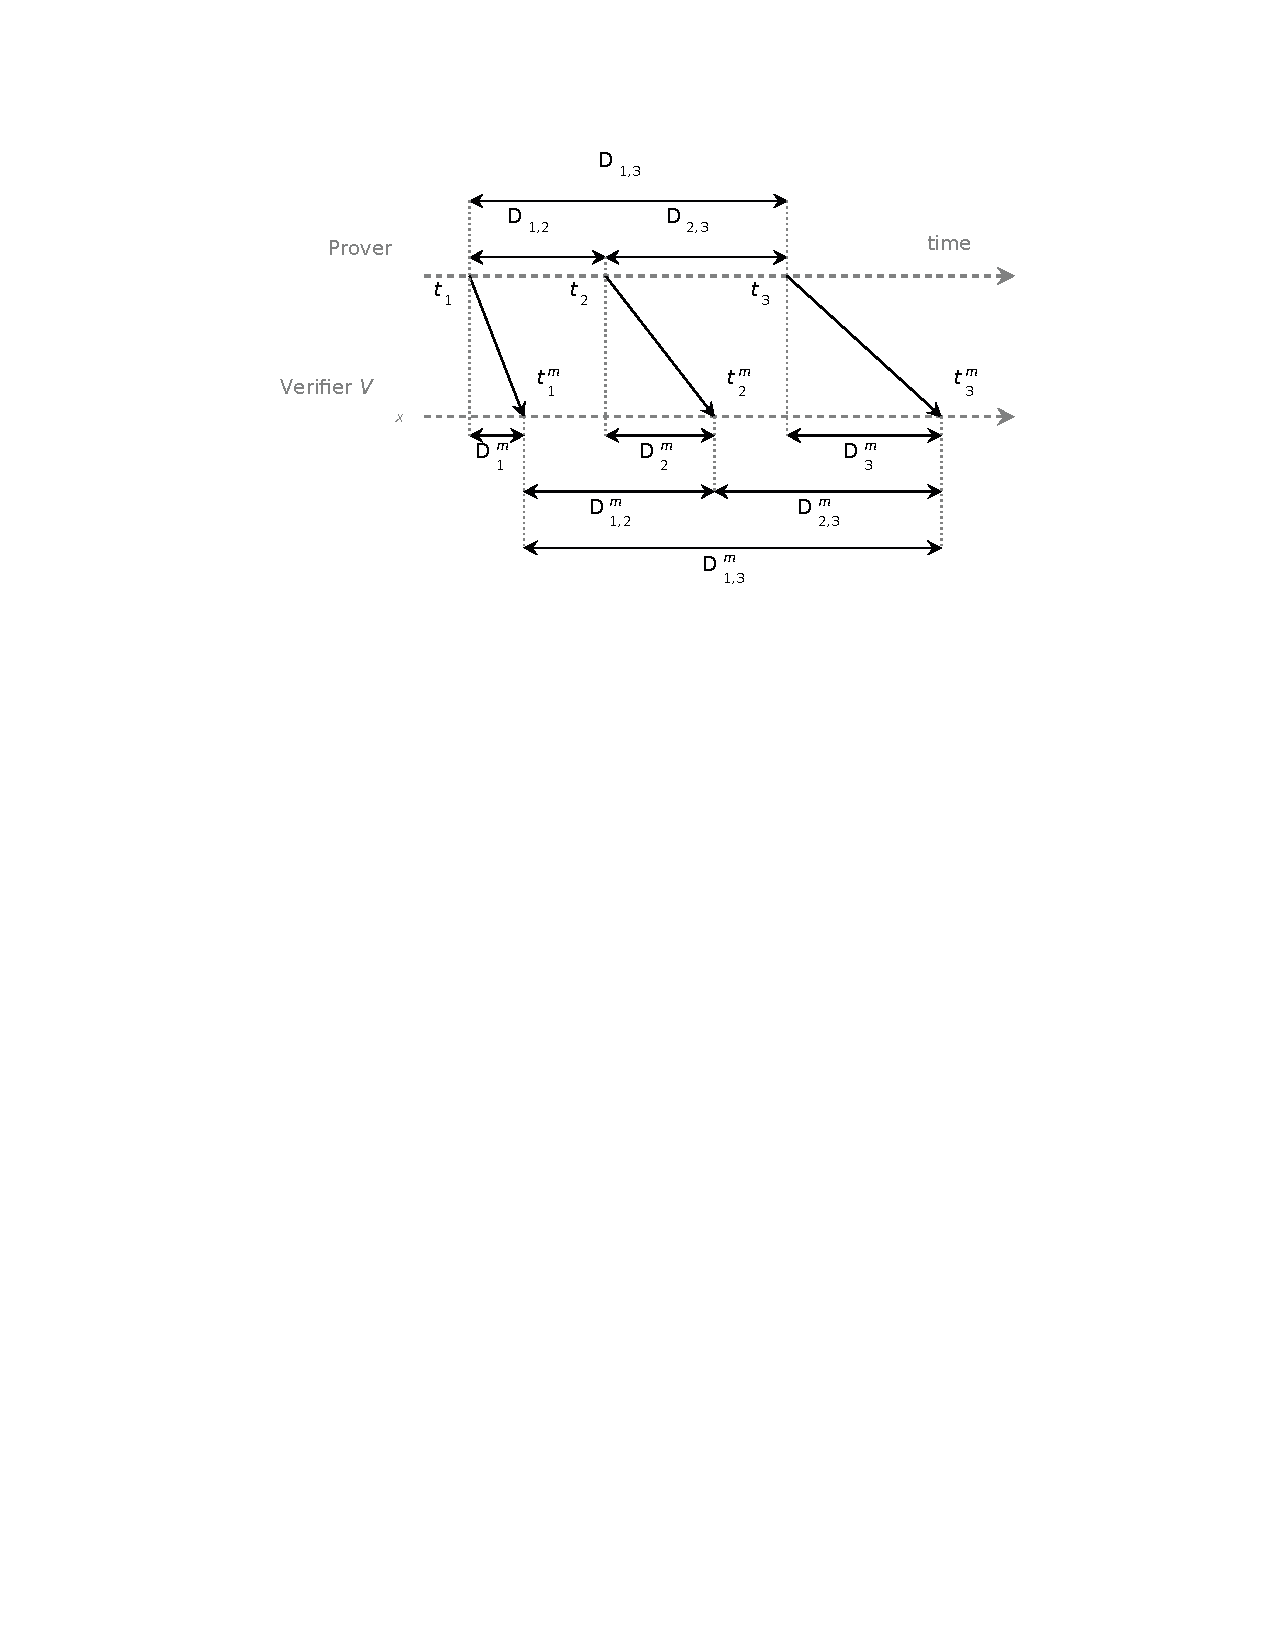
\includegraphics[width=.47\textwidth,trim={46mm 177mm 40mm 20mm},clip]{gm_delay_pic}
    \caption{Delays (noted as \textit{D}) over a timeline for three messages (\textit{1}, \textit{2} and \textit{3})}
    \label{gm_delay_pic}
\end{figure}

\subsection{Frequency Difference of Arrival}

A similar approach can be used exploiting this phenomenon on a frequency domain, where it's known as \textit{Doppler effect}, the physical phenomenon according to which a wave signal (being it sound or light) emitted from one point, can be received with a different frequency if transmitter and receiver are moving relatively to each other (figure \ref{gm_doppler_base}). Indeed depending on direction and speed of the transmitter (here the prover), a specific frequency shift would be measured by the receiver (here the verifier). In an analogous way with respect to the MDToA, a set of equations can be derived from receiver location (known), sender location and speed (both claimed), by means of those is possible to intercept unexpected behaviours. We will refer to this principle as Frequency Difference of Arrival (FDoA) \cite{schaefer16} \cite{ghose15}. The law that must be satisfied by the prover is reported in equations \eqref{gm_radspeed} and \eqref{gm_doppler}.

\begin{equation}
    \label{gm_radspeed}
    v_x = \vec{v} \cdot cos\theta
\end{equation}
\emph{\(v_x\) is the radial speed, which is the component of the prover's speed directed to the verifier. Here \(\theta\) is the angle between the vector \(\vec{v}\) and the verifier position as can be seen in figure \ref{gm_doppler_spd}}

\begin{equation}
    f_m = \frac{f_0}{1-\frac{v_x}{c}}
    \label{gm_doppler}
\end{equation}

\begin{figure}
    \begin{center}
        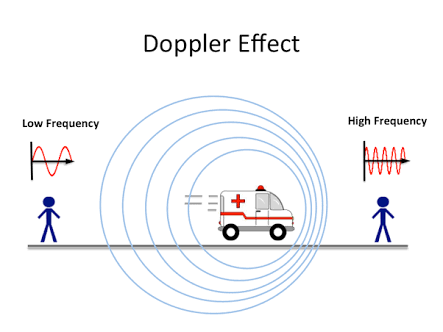
\includegraphics[width=.37\textwidth]{gm_doppler_base.png}
        \caption{The Doppler effect as can be seen considering a sound wave, the same phenomenon happens when dealing with light radiations}
        \label{gm_doppler_base}
    \end{center}
\end{figure}

\begin{figure}
    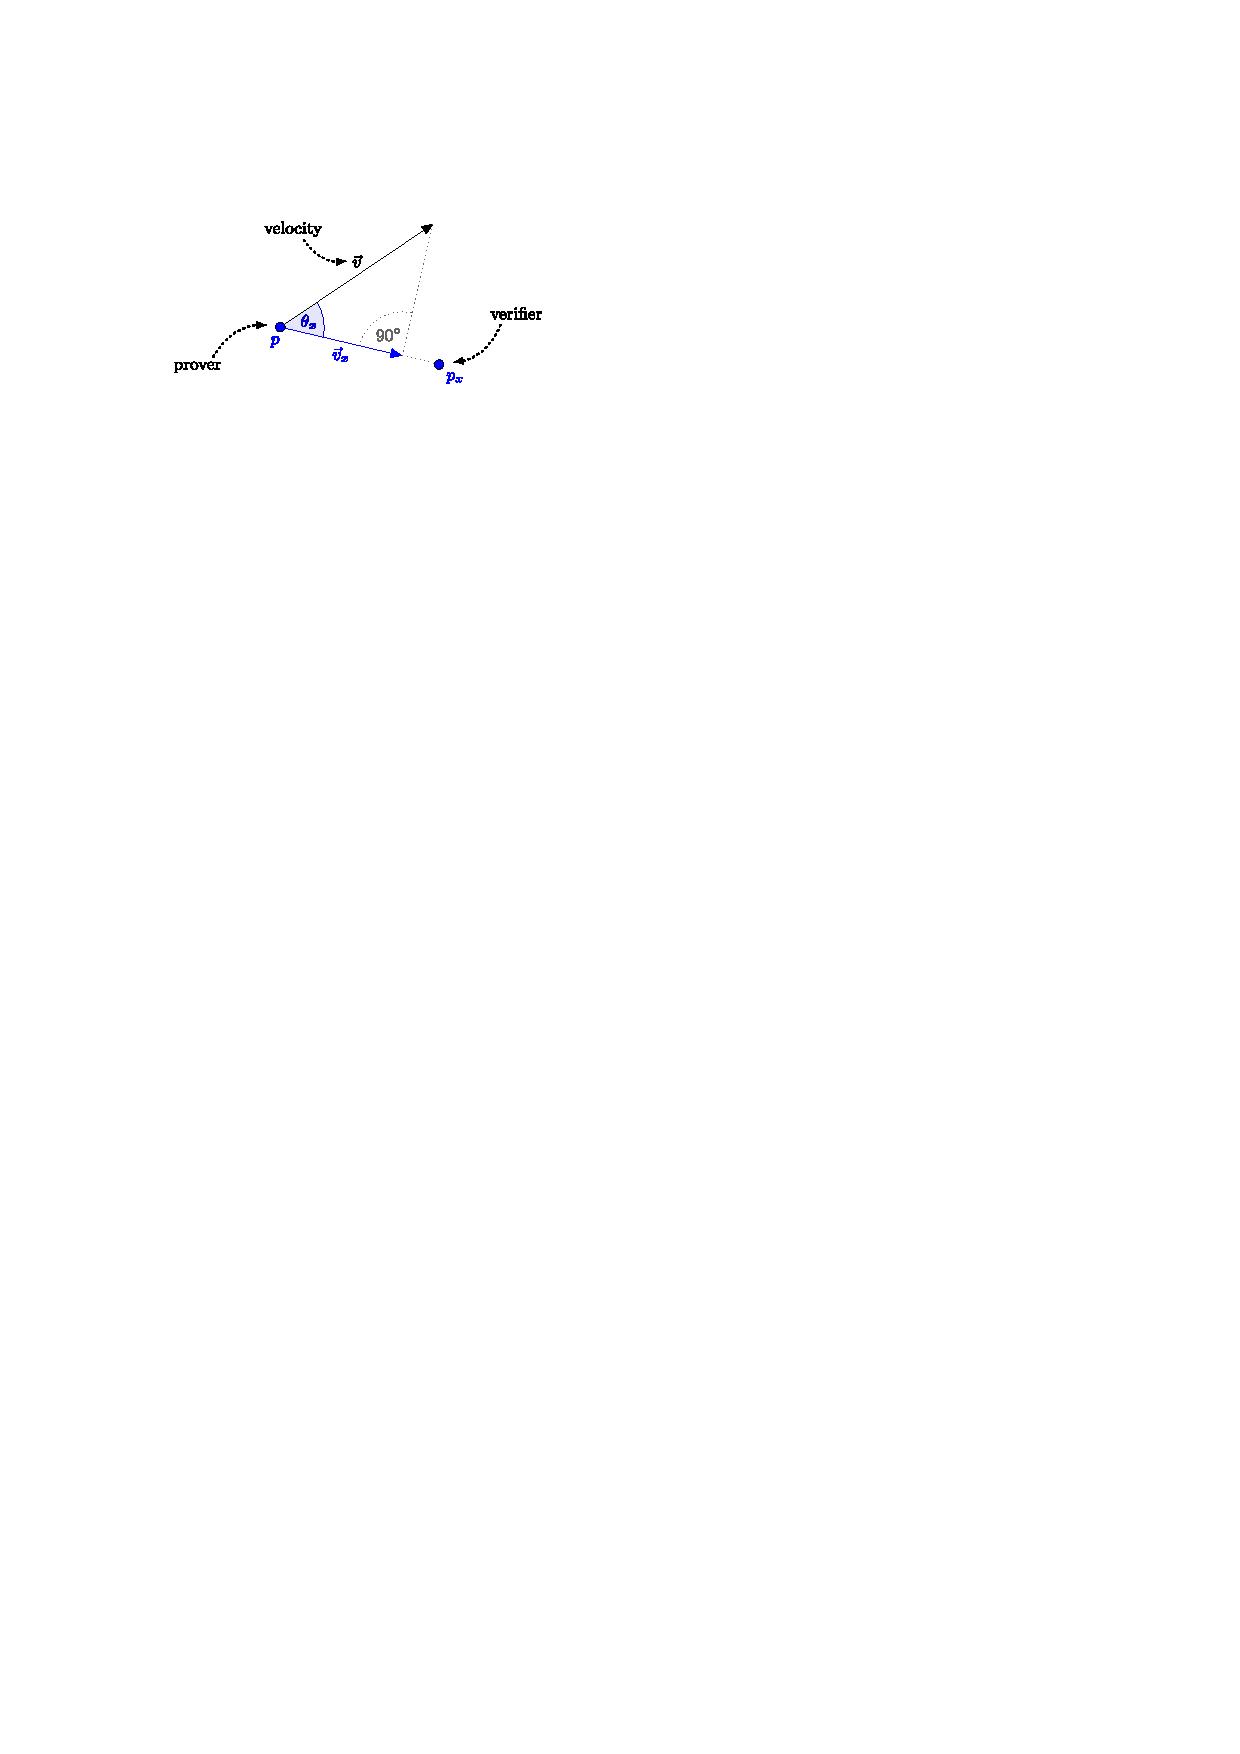
\includegraphics[width=.47\textwidth,trim={27mm 230mm 115mm 35mm},clip]{gm_doppler_spd}
    \caption{Relative speed component used to compute the Doppler effect}
    \label{gm_doppler_spd}
\end{figure}

The verification process, as stated in \cite{schaefer16} and \cite{ghose15}, is carried out by checking the measured frequency \(f_m\) on different location claims against the provided speed and the initial expected frequency. As the formulas are pointing out, we cannot really check the location, since we are only analysing the speed vector, this approach can then be defined as \textit{Motion Verification}. We can then just be sure if the prover is moving as claimed, with respect to our verifier, regardless on it's actual location.

\subsection{Possible attacks and how to cope with them}

While defining both MDToA and FDoA we described a model with one verifier and one prover. In case the prover was actually malicious, we didn't consider it to be aware of the verification system and hence we are not considering it to be able to take any counter measure. Instead it can be proven that, by properly adjusting the delay while sending messages, an attacker can mock it's location and still fulfil the verifier's requirements (\cite{schaefer15} and \cite{schaefer16}).

For instance considering the MDToA case, we suppose an attacker to dispose of a single antenna to transmit its location claims, such attacker would be able to simply add the proper delay while sending beacons and change timestamp on them accordingly (in equation \eqref{gm_delay_trust} we relied on those values) to properly mock it's location to the verifier.

Schäfer et al. \cite{schaefer15} demonstrated that, with the same attacker model involving a single transmitter broadcasting to all the verifiers, simply adding one more verifier is reducing by one degree of freedom the claims the prover can mock. Indeed, while considering the case with a single verifier, the attacker could adjust transmission times and timestamps to virtually mock any track. Instead, by simply adding a new verifier, only some tracks can be successfully spoofed, using the same constructed delays, for both of them.

This trivial modification is drastically improving security, since now the two verifiers can spot suspicious tracks, which may even become unlikely or impossible in some use cases (where the prover is bound to some specific tracks). It is then straightforward to further improve this solution by adding another verifier, which would restrict the usable track by another degree of freedom, a fourth verifier would theoretically even reduce the available track to a single point, which would not be feasible for a mobile prover.
While in theory a set of four verifiers is enough to track down a malicious prover, some additional verifiers may be required in practice to avoid some noise interferences.

A similar conclusion may be derived from the Doppler shift method (as in \cite{schaefer16} and \cite{ghose15}: in this case, the attacker may adapt its transmission frequency to mock the signal for a single verifier, but the addition of more receivers can again reduce the attacker's freedom and eventually make it impossible for a malicious claim to remain undetected, if the verifiers are well placed (e.g. not aligned with each other).

The previously adopted countermeasures only hold under the assumption of an attacker who can use a single transmitter for every verifier, see section %%TODO%%
for further details.

\subsection{Methods in action: Air Traffic Monitoring}

A typical use case of those methods may be aircraft tracking, at the time of writing (2020) the new standard system for locating aircraft, the Automatic Dependent Surveillance-Broadcast (ADS-B), is about to be officially operating to manage air traffic. According to the ADS-B protocol (\cite{adsb}), the airplanes are supposed to know their current parameters (position, speed, etc..) via external systems such as GPS and they are periodically broadcasting such data. Control centers are, instead, gathering all the data related to air traffic and can then control it accordingly. This protocol is expected to be a replacement for classical radar based systems, its implementation is way cheaper and it can be more accurate, but it hasn't been designed with security in mind. Indeed there's no way to verify if received ADS-B packets can be trusted or not.
Costin et al. \cite{costin12} proved that it's not just feasible, but it's also easy with highly available equipments and software, this means that potentially anybody may be able to spoof signals of thousands of \textit{ghost} aircraft, thus making impossible for an airport control center to work and causing severe problems or even danger among real airplanes.

Both MDToA and FDoA can be really helpful in this situation as they both don't require any change on hardware devices on aircraft or in the protocol itself, which is a key feature especially in this field, where a change in protocol may require a full fleet upgrade, which likely would need two decades to become effective (ADS-B has been proposed in the 90s). Indeed those location verification checks are significantly enhancing security by simply exploiting physical properties of the transmission medium, the same control centers reading ADS-B beacons, which are already trusted, can directly be upgraded to also verify the locations of those messages, thus making the solution cheap as well. By exploiting time or frequency \textit{difference} there's even no need to keep time synchronization among verifiers and moreover both the solutions are robust since they are proven to be secure with a certain number of verifiers.

\subsection{Weaknesses and limitations}
As stated earlier, FDoA cannot be used for Track verification but rather for Motion verification, that means that we could spot a malicious attacker only if its speed vector is behaving as expected over time. In this way it can work perfectly against steady attackers, but if also the attacker can move it might be able to successfully spoof its signals. That is however not likely in many applications, since the attacker may need to have a very high speed or to travel along very specific tracks. Besides that, in practice FDoA can be heavily affected by noise in signals, it hence needs a deeper and more refined approach as pointed out by Schäfer et al. \cite{schaefer16}, with their approach analysing multiple location claims can drop to zero the detection error rate.

In addition, Schäfer et al. \cite{schaefer15} suggest that even MDToA can perform worse than expected in real world: it's not guaranteed that all verifiers clocks run with the same speed and their difference might not result as negligible for this purpose. Hence all the errors must be taken into account and the actual performance may be less accurate than expected.

The main limitation of both the methods is related to the fact that we are supposing the verifier to be able to transmit from a single position. Instead, if the attacker could use multiple transmitters, even one for each verifier, and if it could tune the transmission power to avoid all the verifiers to be able to listen to more than one transmitter, it could virtually be able to adjust delays and frequencies separately for each of them. In this way it would be simply impossible to detect the scam and the attacker would be able to spoof any possible position. By all means, that would be a tremendously resource demanding solution, since it would involve many transmitters, properly located and we can assume our attacker model would not reach this depth. It is not likely for the attacker to precisely know all the verifiers position and their reception range, by missing this knowledge it wouldn't be possible to carry on with such a solution.

%% end of my text %%

\begin{thebibliography}{00}
\bibitem{schaefer15} M. Schäfer, V. Lenders and J. Schmitt ``Secure Track Verification,'' 2015 IEEE Symposium on Security and Privacy, San Jose, CA, pp. 199-213, 2015.
\bibitem{schaefer16} M. Schäfer, P. Leu, V. Lenders and J. Schmitt ``Secure Motion Verification using the Doppler Effect,'' Proceedings of the 9th ACM Conference on Security \& Privacy in Wireless and Mobile Networks, pp. 135-145, 2016.
\bibitem{ghose15} N. Ghose and L. Lazos ``Verifying ADS-B navigation information through Doppler shift measurements,'' 2015 IEEE/AIAA 34th Digital Avionics Systems Conference (DASC), pp. 4A2-1, 2015.
\bibitem{costin12} A. Costin and A. Francillon ``Ghost in the Air (Traffic): On insecurity of ADS-B protocol and practical attacks on ADS-B devices,'' Black Hat USA, pp.1-12, 2012.
\bibitem{adsb}ADS-B Info. https://www.ads-binfo.com/. (Time of access; January, 2020)
\end{thebibliography}

\end{document}
